\documentclass[16]{article} %[Tamaño de página y número de fuente]. %Tipo del documento
\usepackage{amsmath} %Añade comandos para ecuaciones
\usepackage[spanish]{babel} %Indica idioma del documento
\usepackage[utf8]{inputenc} %Permite escribir caracteres particulares del español (tildes, ñ, ...). Equivalente a poner \'a
\usepackage{vmargin} %Para editar márgenes
\usepackage{graphicx} %Permite instertar imágenes
\usepackage{tikz} %Permite insertar elementos gráficos

\begin{document} %Crea el entorno del documento
\begin{titlepage} %Portada
	\centering  %Centra el texto
	{\bfseries\Huge Teoría de Autómatas y Lenguajes Formales\par}
   	\vspace{2cm} %Crea un espacio vertical
    {\bfseries\huge Actividades Práctica 2\par}
    \vfill %Rellena el espacio para ocupar la página entera
    {\huge Iván Romero Molina\par}
    \vspace{1cm}
    {\Large Universidad de Málaga\par}
    \vspace{1cm}
    {\large 30 de octubre de 2022\par}
\end{titlepage}
    
\newpage
%\thispagestyle{empty} Quita el número de página
\section*{\huge Enunciado}
\noindent %Quita el sangrado de un párrafo
Consideraremos el lenguaje sobre el alfabeto $\{a, b\}$ que solo contenga la cadena a.
\section*{Apartado 1}	%Si tiene * quita la numeración
\noindent
Descripción matemática del autómata:
Sea $M=(\{q_0,q_1,q_2\}, \{a,b\}, \delta, q_0, \{q_1\})$ un AFD con
\begin{table}[h!]
	\begin{tabular}{c|c|c}
  	$\delta(q,\sigma)$ & $a$ & $b$\\
  	\hline
  	$q_0$& $q_1$ & $q_2$\\
  	\hline
  	$q_1$& $q_2$ & $q_2$\\
  	\hline
  	$q_2$& $q_2$ & $q_2$
	\end{tabular}
\end{table}
\\
\section*{Apartado 2}
\noindent
Hacer el autómata que reconozca el lenguaje y rechaze todas aquellas cadenas que no pertenezcan a dicho lenguaje en JLFAP. Además, se prueba el autómata introduciendo 6 cadenas:\\\\
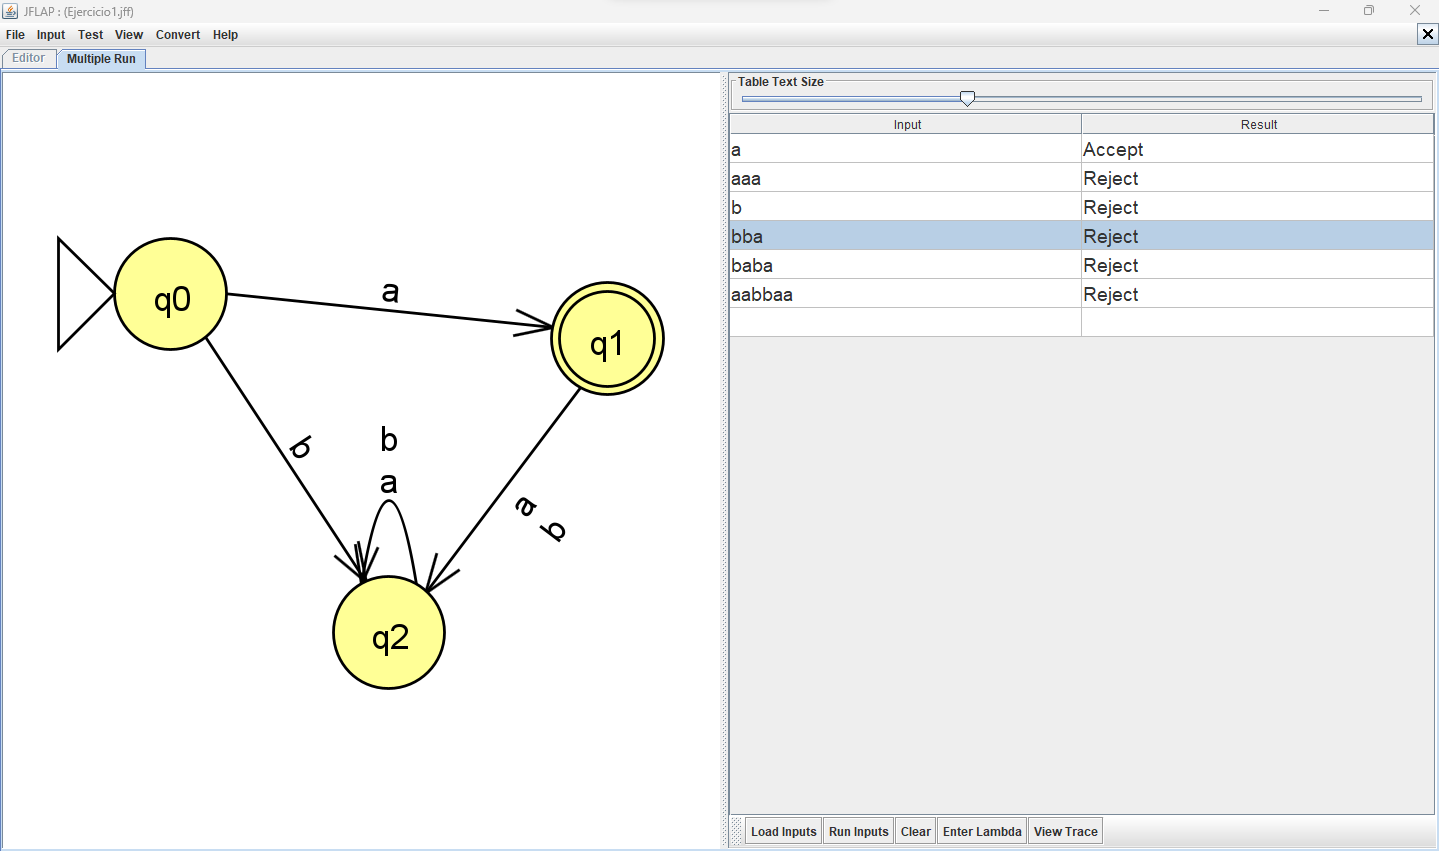
\includegraphics[width=1.1\linewidth]{Apartado2.png}

\newpage
\section*{Apartado 3}
\noindent
Describir el JSON en Octave:\\\\
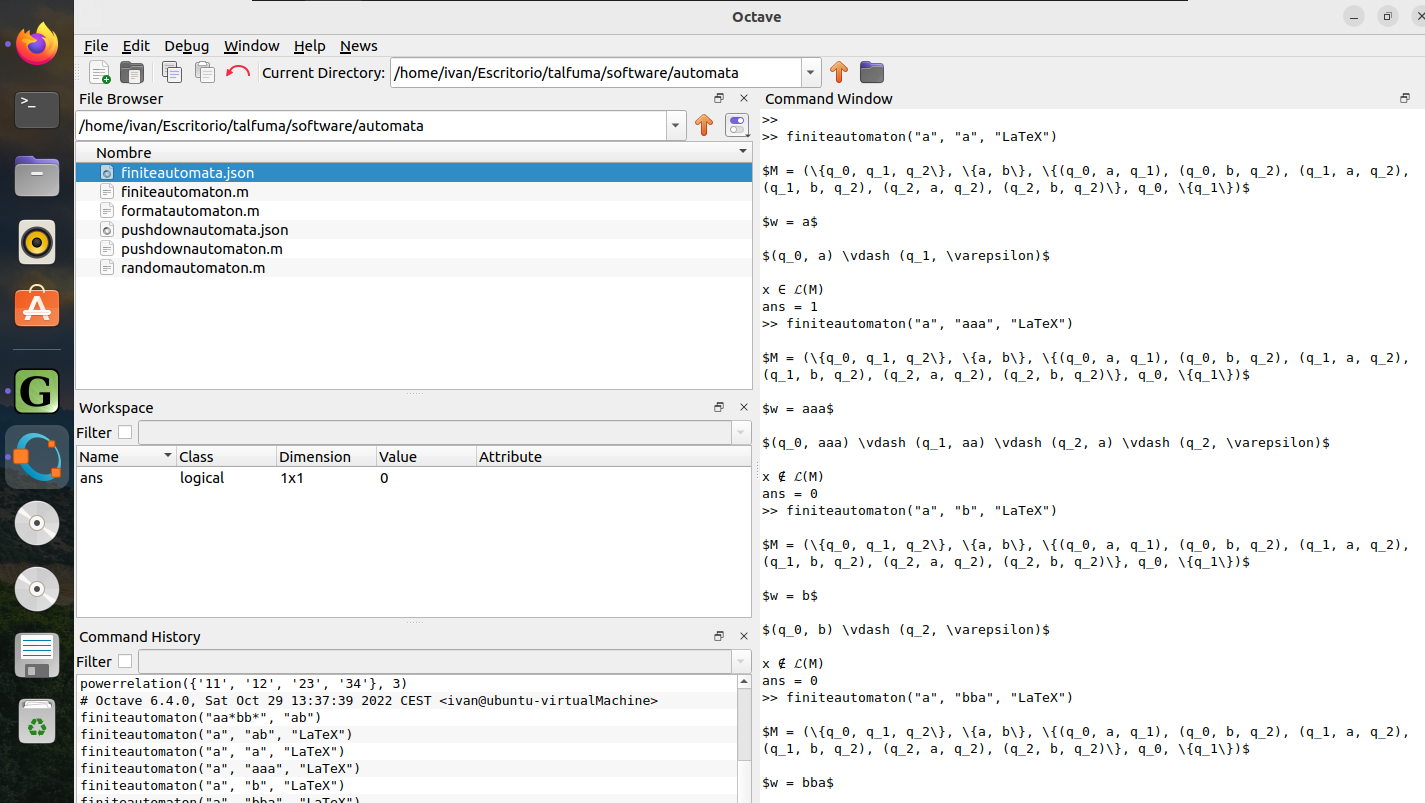
\includegraphics[width=1.1\linewidth]{Apartado3a.png}
\\\\
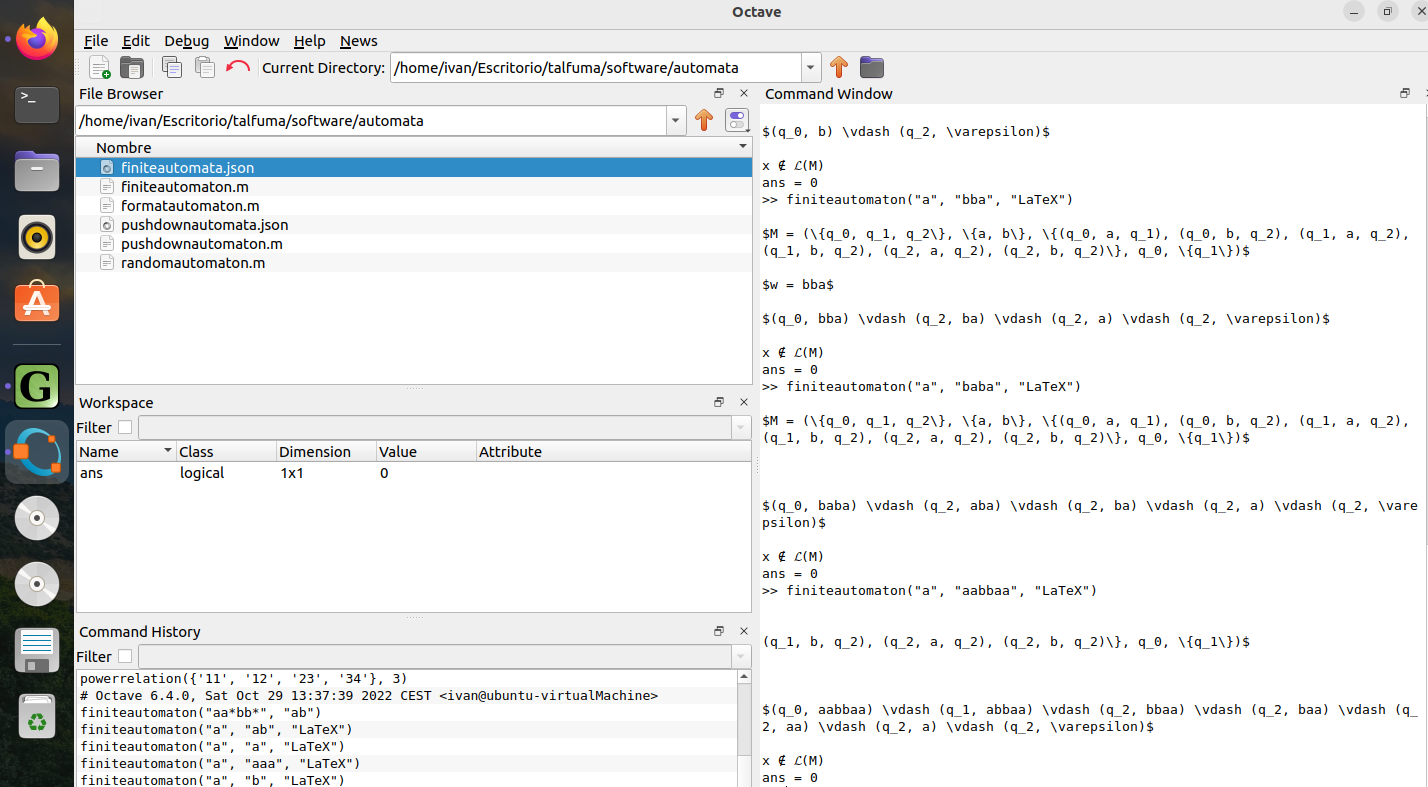
\includegraphics[width=1.1\linewidth]{Apartado3b.png}
\end{document}